\documentclass[a4paper]{article}
% useful packages.
\usepackage{authblk}
\usepackage{amsfonts}
\usepackage{amsmath}
\usepackage{amssymb}
\usepackage{amsthm}
\usepackage{enumerate}
\usepackage{graphicx}
\usepackage{multicol}
\usepackage{fancyhdr}
\usepackage{layout}
\usepackage{float}
\usepackage{subcaption}
\newtheorem{Definition}{\hspace{2em}定义}
\newtheorem{Example}{\hspace{2em}例}
\newtheorem{Thm}{\hspace{2em}定理}
\newtheorem{Lem}{\hspace{2em}引理}
\newtheorem{cor}{\hspace{2em}推论}
% some common command
\newcommand{\dif}{\mathrm{d}}
\newcommand{\avg}[1]{\left\langle #1 \right\rangle}
\newcommand{\difFrac}[2]{\frac{\dif #1}{\dif #2}}
\newcommand{\pdfFrac}[2]{\frac{\partial #1}{\partial #2}}
\newcommand{\OFL}{\mathrm{OFL}}
\newcommand{\UFL}{\mathrm{UFL}}
\newcommand{\fl}{\mathrm{fl}}
\newcommand{\op}{\odot}
\newcommand{\cp}{\cdot}
\newcommand{\Eabs}{E_{\mathrm{abs}}}
\newcommand{\Erel}{E_{\mathrm{rel}}}
\newcommand{\DR}{\mathcal{D}_{\widetilde{LN}}^{n}}
\title{Report For Discontinuous Galerkin Method}
\author{Shuang Hu}
\affil{Zhejiang University}
\begin{document}
\maketitle
\section{Problem Statement}
Using the third-order DG scheme to solve the Burgers' equation 
\begin{equation}
    \left\{
    \label{eq:Burgers}
    \begin{aligned}
        u_{t}+uu_x&=0,\\
        u(x,0)&=g(x)=1/2+\sin(x),\quad 0\le x\le 2\pi,
    \end{aligned}
    \right.
\end{equation}
with periodic boundary condition. This report will contain the following contents:
\begin{itemize}
    \item Derive the exact solution of Burgers equation \eqref{eq:Burgers}.
    \item Algorithm design and some related properties.
    \item Numerical results.
    \item Discussions.
\end{itemize}
\section{Burgers' equation}

In this section, we will introduce some theoretical results for Burgers' equation. 

Choose the \textbf{flux} $f(u):=\frac{u^2}{2}$, Burgers' equation is a special type of the 
1D conservation law:
\begin{equation}
    \label{eq:conservationlaw}
    \left\{
    \begin{aligned}
        u_{t}+(f(u))_{x}&=0,\\
        u(x,0)&=g(x).\\
    \end{aligned}
    \right.
\end{equation}
Consider the curve $y=\eta(t;x_{0})$ satisfying:
\begin{equation}
    \label{eq:Char_line}
    \begin{aligned}
        \eta'(t;x_{0})&=u(\eta(t;x_{0}),t),\\
        \eta(0)&=x_{0},\\
    \end{aligned}
\end{equation}
along the curve $\eta(t;x_0)$, equation \eqref{eq:Burgers} 
is equivalent to 
\begin{equation}
    \label{eq:Characteristic_cons_law}
    \left\{
    \begin{aligned}
        \frac{\dif}{\dif t}u(\eta(t;x_{0}),t)&=0,\\
        u(x_{0},0)&=g(x_{0}).
    \end{aligned}
    \right.
\end{equation}
It means that $u(x,t)$ remains constant along the curve 
$\eta(t;x_{0})$, and the curve $y=\eta(t;x_{0})$ is the \textbf{characteristic line} 
for equation \eqref{eq:Burgers}.

So, we find the solution $u(x,t)$ by the following two steps:
\begin{itemize}
    \item Derive a characteristic line $y=\eta(t;\xi)$ from equation \eqref{eq:Char_line}, 
    which passes through the point $(x,t)$.
    \item Set $u(x,t):=g(\xi)$.
\end{itemize}
By \eqref{eq:Char_line}, $\eta(t;\xi)=\xi+g(\xi)t$, i.e. 
\begin{displaymath}
    x=\xi+ut.
\end{displaymath}
Then we can derive the solution as an implicit form:
\begin{equation}
    \label{eq:sol_of_Burgers}
    u(x,t)=g(x-u(x,t)t).
\end{equation}
If the characteristic lines don't intersect for $t\in[0,T]$, 
the equation \eqref{eq:Burgers} is well-posed. 
Unfortunately, it isn't still true for each $T>0$. Here is the characteristic lines 
if we choose $T=1.2$.
\begin{figure}[H]
    \centering
    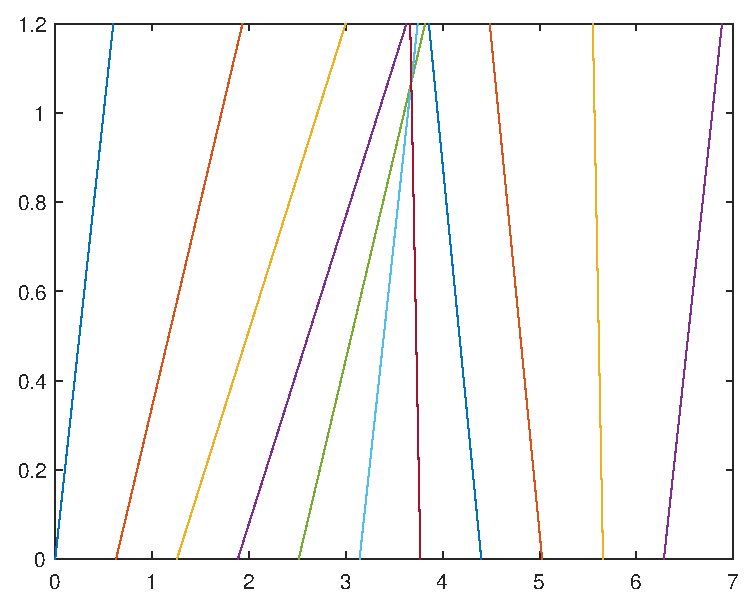
\includegraphics[width=\linewidth,height=6cm]{figure/Charline.eps}
    \caption{Characteristic lines.}
\end{figure}
If the characteristic lines intersect with each other, it means that 
equation \eqref{eq:Burgers} has no strong solutions, and its weak solutions are 
\textbf{discontinuous}. By \cite[Exercise 3.3]{1}, the solution will break at time 
\begin{equation}
    T_{b}=\frac{-1}{\min g'(x)}=1.
\end{equation}
And the discontinuous point will move forward as well, which forms a \textbf{shock wave}. 
The entropy weak solution is a strong solution on both sides of the shock wave, 
and discontinuous on the shock wave points. 
In this problem, the shock wave originates from $x_{0}=\pi$ with the speed 
\begin{equation}
    s=\frac{g(x_{0}^-)+g(x_{0}^{+})}{2}=0.5,
\end{equation}
see \cite[(3.26)]{1}.
\section{Algorithm}
In this section, we introduce the DG scheme briefly with some tricks for implementation.

\subsection{Mesh and finite element space}
In this assignment, we choose equidistant grids. Assume there are $N$ elements on the 
interval $[0,2\pi]$, mark $h:=\frac{2\pi}{N}$, the $j-th$ element is 
\begin{displaymath}
    I_{j}:=[x_{j-\frac{1}{2}},x_{j+\frac{1}{2}}]
    =\left[\frac{2\pi(j-1)}{N},\frac{2\pi j}{N}\right],
\end{displaymath}
and the finite element space 
\begin{displaymath}
    V_{h}^{2}:=\{u\in L^{2}([0,2\pi]):u|_{I_j}\in P^{2}(I_j)\}.
\end{displaymath}
$P_{2}(I_{j})$ is the vector space of all polynomials on 
$I_{j}$ with degree less than or equal to 2. 
We choose the Legendre-form basis for $P_{2}(I_{j})$, i.e. 
\begin{equation}
    \label{eq:basis}
    \begin{aligned}
        P_{2}(I_j)&=\text{span}\{p_{j}^{0},p_{j}^{1},p_{j}^2\},\\
        p_{j}^{0}&=1,\quad p_{j}^{1}=\frac{1}{h}\left(x-\frac{x_{j}+x_{j+1}}{2}\right),\\
        p_{j}^{2}&=\frac{3}{2}\left(\frac{2x-x_{j}-x_{j+1}}{h}\right)^2-\frac{1}{2}.
    \end{aligned}
\end{equation}
It's an orthogonal basis for $P_{2}(I_j)$.
\subsection{Weak form and finite element approximation}
Now derive the weak form for \eqref{eq:conservationlaw}. Choose $v\in V_{h}^{2}$, 
integration by parts on $I_{j}$, we get:
\begin{equation}
    \label{eq:one_elem_weak_form}
    \int_{I_j}u_t v\dif x-\int_{I_j}f(u)v_x\dif x+f(u)v|_{x_{j+\frac{1}{2}}^{-}}
    -f(u)v|_{x_{j-\frac{1}{2}}^{+}}, \forall u\in V_{h}^{2}.
\end{equation}
Since $u$ maybe discontinuous on $x_{j\pm\frac{1}{2}}$, we use 
\textbf{numerical flux} to substitute $f(u)|_{x_{j\pm\frac{1}{2}}}$. 
In this assignment, we choose \textbf{Lax-Friedriches flux}:
\begin{equation}
    \label{eq:LFflux}
    \hat{f}^{LF}(u^{+},u^{-}):=\frac{1}{2}
    \left(f(u^-)+f(u^+)-\alpha(u^{+}-u^{-})\right),
    \quad \alpha=\max_{u}|f'(u)|.
\end{equation}
Then, choose $u_{j}:=c_{j}^{0}(t)p_{j}^{0}+c_{j}^{1}(t)p_{j}^{1}+c_{j}^{2}(t)p_{j}^{2}$, 
$v_{j,i}:=p_{j}^{i}$, \eqref{eq:one_elem_weak_form} and \eqref{eq:LFflux} 
derive a semi-discretize numerical scheme.

The Lax-Friedriches flux \eqref{eq:LFflux} is \textbf{consistent, Lipschitz 
continuous and monotone}, so this scheme satisfies discretize entropy inequality, 
see \cite{2}.

In fact, since $(p_{i}^{2},p_{j}^{2})_{L^{2}(I_j)}=k\delta_{ij}$, the mass matrix of 
\eqref{eq:one_elem_weak_form} is just a diagonal matrix. 
So this scheme is efficient.
\subsection{Time Integration}
In this assignment, we use \textbf{TVD Runge-Kutta scheme} to solve 
the ODE system $U_{t}=\mathcal{L}(U)$:
\begin{equation}
    \label{eq:TVD-RK}
    \begin{aligned}
    U^{(1)}&=U^{n}+\Delta t\mathcal{L}(U^{n}),\\
    U^{(2)}&=\frac{3}{4}U^{n}+\frac{1}{4}(U^{(1)}+\Delta t\mathcal{L}(U^{(1)})),\\
    U^{n+1}&=\frac{1}{3}U^{n}+\frac{2}{3}(U^{(2)}+\Delta t\mathcal{L}(U^{(2)})).\\
    \end{aligned}
\end{equation}
\section{Numerical Result}
In this section, we will give the numerical results.
\subsection{Before break time}
First, we test the $L^{1}$, $L^{\inf}$ error and convergence rates for this numerical scheme. 
We choose $T=0.2$, $N=20,40,80,160,320$ and $k=0.1h$. Here are the results.
\begin{table}[H]
    \begin{tabular}{llllllllll}
        \hline
                          & 20      & rate & 40      & rate & 80      & rate & 160     & rate & 320     \\ \hline
        $L^{1}$ norm      & 8.18e-4 & 2.82 & 1.16e-4 & 2.76 & 1.71e-5 & 2.75 & 2.53e-6 & 2.75 & 3.77e-7 \\
        $L^{\infty}$ norm & 1.10e-3 & 2.60 & 1.81e-4 & 2.62 & 2.95e-5 & 2.66 & 4.69e-6 & 2.67 & 7.38e-7 \\ \hline
    \end{tabular}   
    \caption{The error and convergence rate} 
\end{table} 
In this test, we choose $\alpha=1.5$ for the Lax-Friedriches flux, and use 
Newton's method to derive the solution of Burgers' equation. We write the 
modified equation 
\begin{displaymath}
    w=\sin(x-wt-\frac{t}{2}),\quad u=w+\frac{1}{2},
\end{displaymath}
and set the initial value $w=0.8$ beyond the shock wave, i.e. $x<\pi+0.5t$, the initial value 
$w=-0.8$ after the shock wave, i.e. $x>\pi+0.5t$.
\subsection{After break time}
In this section, we give some figures for $T=0,0.5,1,1.5$ to show the continuous 
and discontinuous solutions.
\begin{figure}[H]  
    \centering  
    \begin{subfigure}{0.45\textwidth}  
        \centering  
        \includegraphics[width=\textwidth,height=2.5cm]{figure/Burgers(1).eps}  
        \caption{$T=0$}  
        \label{fig:initial}  
    \end{subfigure}  
    \hfill  
    \begin{subfigure}{0.45\textwidth}  
        \centering  
        \includegraphics[width=\textwidth,height=2.5cm]{figure/Burgers(2).eps}  
        \caption{$T=0.5$}  
        \label{fig:BurgersT0.5}  
    \end{subfigure}  
    \vskip\baselineskip  
    \begin{subfigure}{0.45\textwidth}  
        \centering  
        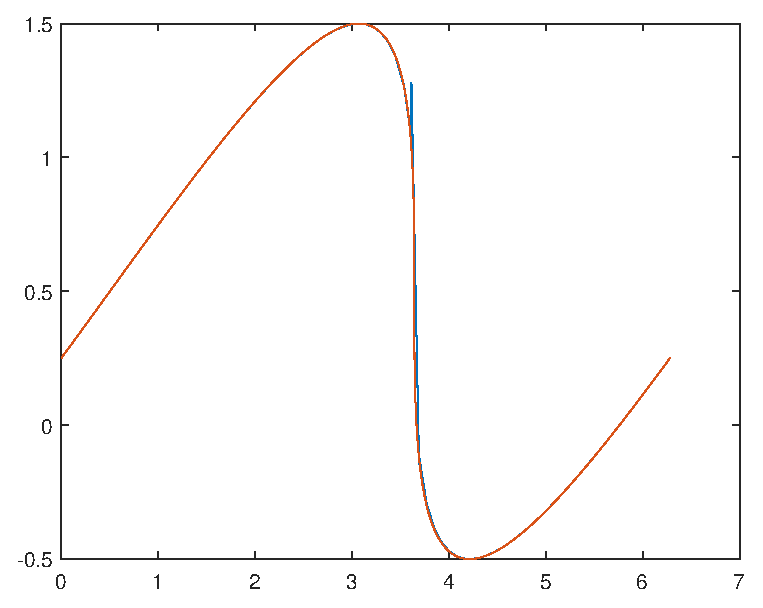
\includegraphics[width=\textwidth,height=2.5cm]{figure/Burgers(3).eps}  
        \caption{$T=1$}  
        \label{fig:BurgersT1}  
    \end{subfigure}  
    \hfill  
    \begin{subfigure}{0.45\textwidth}  
        \centering  
        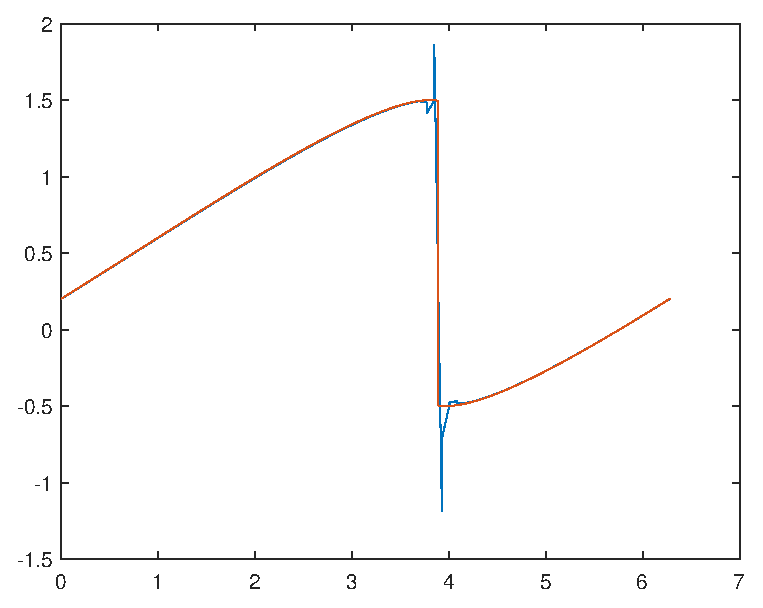
\includegraphics[width=\textwidth,height=2.5cm]{figure/Burgers(4).eps}  
        \caption{$T=1.5$}  
        \label{fig:BurgersT1.5}  
    \end{subfigure}  
    \caption{The numerical solution of Burgers equation}  
    \label{fig:main}  
\end{figure}  
The red lines are the exact solutions, and the blue lines are the numerical solutions.  
Severe oscullations occur for $T>1$, which means the $P_2$ element DG method isn't 
TV(Total Variation) stable. 

Now, we try to operate the limiter introduced in \cite[Section 3.2.2]{2}. 
After we operate the limiter, we eliminate the oscullations. It shows:
\begin{figure}[H]  
    \centering  
    \begin{subfigure}{0.45\textwidth}  
        \centering  
        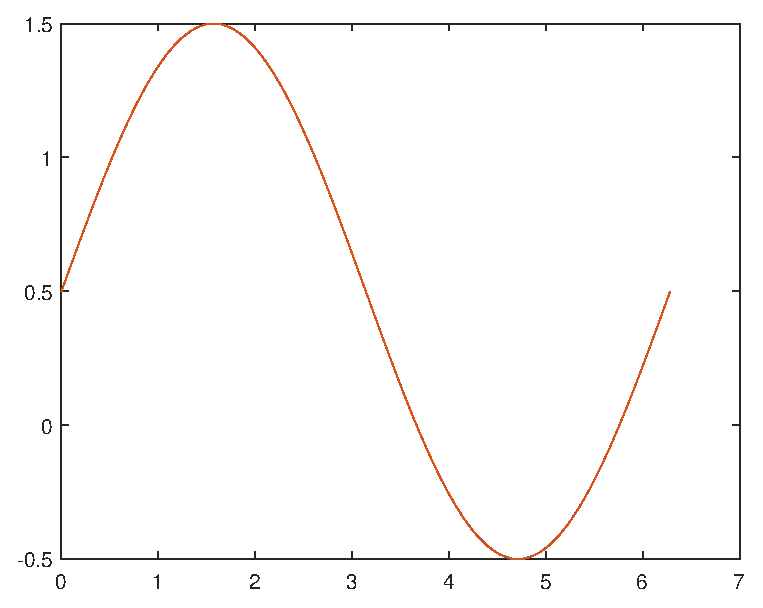
\includegraphics[width=\textwidth,height=2.5cm]{figure/AdjBurgers(1).eps}  
        \caption{$T=0$}  
        \label{fig:initial}  
    \end{subfigure}  
    \hfill  
    \begin{subfigure}{0.45\textwidth}  
        \centering  
        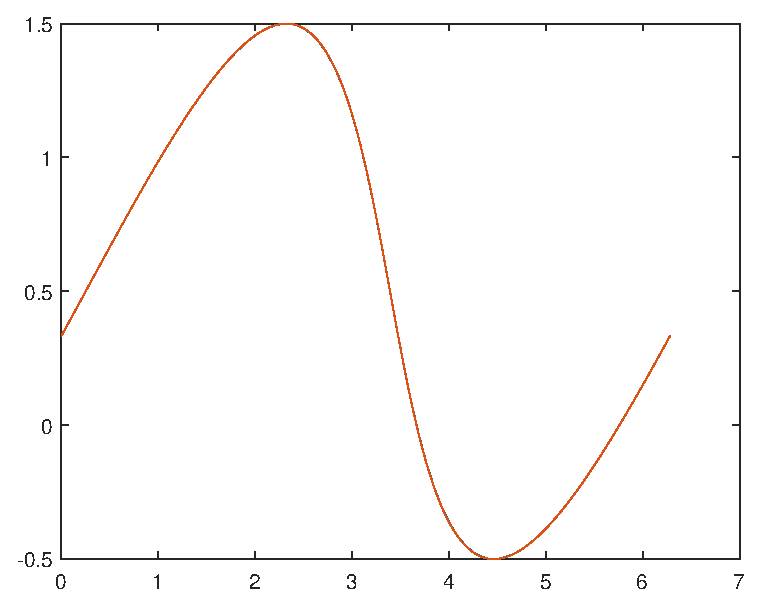
\includegraphics[width=\textwidth,height=2.5cm]{figure/AdjBurgers(2).eps}  
        \caption{$T=0.5$}  
        \label{fig:BurgersT0.5}  
    \end{subfigure}  
    \vskip\baselineskip  
    \begin{subfigure}{0.45\textwidth}  
        \centering  
        \includegraphics[width=\textwidth,height=2.5cm]{figure/AdjBurgers(3).eps}  
        \caption{$T=1$}  
        \label{fig:BurgersT1}  
    \end{subfigure}  
    \hfill  
    \begin{subfigure}{0.45\textwidth}  
        \centering  
        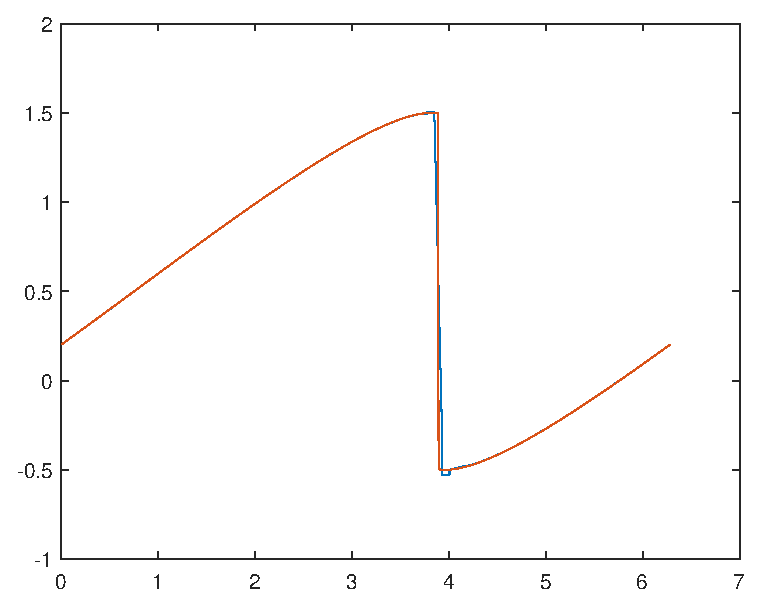
\includegraphics[width=\textwidth,height=2.5cm]{figure/AdjBurgers(4).eps}  
        \caption{$T=1.5$}  
        \label{fig:BurgersT1.5}  
    \end{subfigure}  
    \caption{The numerical solution of Burgers equation after limiter}  
    \label{fig:main}  
\end{figure}  
These figures show that the numerical solutions fit the actual solution of Burgers' equation 
well.
\section{Discussions}
Now, we make some discussions for the numerical results. 
\begin{itemize}
    \item By \eqref{eq:LFflux}, we should choose $\alpha=1.5$. 
    But for $\alpha=0$ or $\alpha=1$, the scheme also works, even gives better numerical 
    result, why?
    \item How to make a prior estimation for the parameter $\alpha$?
    \item In this assignment, we generate the initial value by interpolation method 
    on $x_{j-\frac{1}{2}},x_{j+\frac{1}{2}},\frac{x_{j-\frac{1}{2}}+x_{j+\frac{1}{2}}}{2}$. 
    If we try $L^{2}$-projection method to generate the initial value, things will 
    different or not?
    \item In practise, we use the limiter for the final result, and the shock wave 
    eliminates, why? 
    \item The limiter operator limits $u(x_{j-\frac{1}{2}}^{+})$ and $u(x_{j+\frac{1}{2}}^{-})$, 
    but I'm not sure how to get $\tilde{u}_{I_{j}}$ from this modified values. 
    I set $\tilde{u}_{I_j}$ as the linear function, but the result seems not true. 
    How to deal with this problem?
\end{itemize}
\begin{thebibliography}{99}
    \bibitem{1} Randall J.Leveque, Numerical Methods for Conservation Laws.
    \bibitem{2} Chi-Wang Shu, Discontinuous Galerkin Methods: General Approach and Stability.
\end{thebibliography}
\end{document}